\documentclass[preprint]{aastex62}

\newcommand{\vdag}{(v)^\dagger}
\newcommand\aastex{AAS\TeX}
\newcommand\latex{La\TeX}

%% Tells LaTeX to search for image files in the 
%% current directory as well as in the figures/ folder.
\graphicspath{{./}{figures/}}


%% Reintroduced the \received and \accepted commands from AASTeX v5.2
\received{October 18, 2018}
\revised{---}
\accepted{---}
%% Command to document which AAS Journal the manuscript was submitted to.
%% Adds "Submitted to " the arguement.
% \submitjournal{ApJ}

\shorttitle{Alternative Theories}
\shortauthors{Kavelaars et al.}

%\watermark{NRC-DRAFT}

\begin{document}

\title{Perspectives on the distribution of orbits of distant Trans-Neptunian Objects}

\correspondingauthor{J. J. Kavelaars}
\email{JJKavelaars@gmail.com}
\author[0000-0001-7032-5255]{J. J. Kavelaars}
\affil{Department of Physics and Astronomy, University of Victoria, Elliott Building, 3800 Finnerty Rd, Victoria, BC V8P 5C2, Canada}
\affil{Herzberg Astronomy and Astrophysics Research Centre, National Research Council of Canada, 5071 West Saanich Rd, Victoria, British Columbia V9E 2E7, Canada}


\author[0000-0001-5368-386X]{Samantha M. Lawler}
\affil{Herzberg Astronomy and Astrophysics Research Centre, National Research Council of Canada, 5071 West Saanich Rd, Victoria, British Columbia V9E 2E7, Canada}

\author[0000-0003-3257-4490]{Michele T. Bannister}
\affiliation{Astrophysics Research Centre, School of Mathematics and Physics, Queen's University Belfast, Belfast BT7 1NN, United Kingdom}

\author[0000-0002-3507-5964]{Cory Shankman}
\affiliation{Department of Physics and Astronomy, University of Victoria, Elliott Building, 3800 Finnerty Rd, Victoria, BC V8P 5C2, Canada}


\begin{abstract}

Hello, that was abstract. 

\end{abstract}

%% Keywords should appear after the \end{abstract} command. 
%% See the online documentation for the full list of available subject
%% keywords and the rules for their use.
\keywords{Kuiper belt, orbits --- biases ---  surveys}

%% From the front matter, we move on to the body of the paper.
%% Sections are demarcated by \section and \subsection, respectively.
%% Observe the use of the LaTeX \label
%% command after the \subsection to give a symbolic KEY to the
%% subsection for cross-referencing in a \ref command.
%% You can use LaTeX's \ref and \label commands to keep track of
%% cross-references to sections, equations, tables, and figures.
%% That way, if you change the order of any elements, LaTeX will
%% automatically renumber them.
%%
%% We recommend that authors also use the natbib \citep
%% and \citet commands to identify citations.  The citations are
%% tied to the reference list via symbolic KEYs. The KEY corresponds
%% to the KEY in the \bibitem in the reference list below. 


\section{Introduction}

Looking at the orbits of small bodies at large semimajor axis we are compelled to see
patterns. Some of those patterns are noted as strong
indicators of new or hidden processes in the outer Solar System,
others are substantially observational biases, and still others are
completely overlooked. We can gain insight into the current and past
structure of the outer Solar System through a careful examination of
these orbit patterns.

In this chapter we discuss the implications that can be taken from the observed distant trans-Neptunian object (TNO) orbital distribution.  We start with some cautions on observational biases inherent in the population of known TNOs.  Some of these biases are intrinsic to the process of discovering TNOs while others can be reduced or eliminated through careful observational survey design. We then discuss some orbital element correlations that have received considerable attention in the recent literature. We then examine the known TNOs in the context of the gravitational processes the known Solar System induces in the orbital distribution of the known Kuiper belt.  We then discuss proposed new elements to the outer Solar System and posited ancient processes and the types of orbital element distributions they predict to exist.  We conclude with speculation.

\section{Biases in detection of distant solar system objects.}
\label{sec:intro}

We perceive the reality of the universe through our observation of that universe, and our understanding of those observations are biased by our observation and perception biases. This truism of observational science must be kept in mind when considering the review of our data. As a group, we examine data and look for meaning in the correlations between quantities and strongly cling to our initial conceptions.  To see beyond our perception biases is difficult and perhaps intractable. 

The Kuiper belt is over 4.5 billion km distant from the Earth-bound observer, with the most distant objects known being three times further away still.  The challenge of detecting objects at these great distances should not be under-estimated.  The Sun's light reflected off Solar System bodies is dimmed by $r^{-4}$, greatly exaggerating our sensitivity to nearby sources in comparison to more distant objects.  The volume of the Solar neighbourhood that a survey is sensitive to, its {\it detection volume},  is, at minimum, limited in radial extent. The strength of the $r^{-4}$ observational bias is frequently under-appreciated when attempting to interpret the distributions of objects detected by a particular survey.

Objects on orbits with moderate to large eccentricities also present a distorted view of the population.  Those objects occupy a range of solar distances, resulting in a time-variable $r^{-4}$-flux bias. An object may only spend a small fraction of its orbital period within the detection volume of a particular survey. The larger the semi-major axis, the larger the eccentricity needed to bring the object within the detection volume and the smaller the fraction of the orbit that object remains in that volume of space.

Limited telescopic resources add another layer of complexity to the problem of seeing the biases inherent in the detected sample of TNOs.  Essentially, one can only detect objects in the part of the sky where one looks.  This observer direction bias imposes a relation between the Nodal angle ($\Omega$), argument of pericentre ($\omega$), mean anomaly ($\mathcal{M}$) and inclination ($i$) of an orbit that can be detected.  This coupling of multiple angles can be difficult to conceptualize.  For illustration, consider a discovery survey whose fields all straddle the ecliptic plane.  In those surveys,  orbits that are inclined to the ecliptic plane and have an inclination that is exceeds the latitude sensitivity of the survey will only be visible when looking towards their nodes. Combine the forced detection at the node with the preferential discovery of objects near their peri-centre (caused by the $r^{-4}$ flux bias discussed above) and such a the survey will find that the detected sample of objects on inclined orbits all have arguments of pericentre $\omega$ near 0 and 180$^{\circ}$. This effect is well known and is described here to remind the reader of the basic processes at work.  When attempting to maximize the science return of scarce observing time, by observing fields in specific areas of sky, one induces biases in the detected sample that may be difficult to recognize. 

In Figure~\ref{fig:bias} we present the orbital distribution of a subsample of objects reported to the Minor Planet Centre (as of 2018-Oct-15). This figure presents all TNOs (dots) with $a > 150$~au and $q > 30$~au.  The vertical line at 1000~au {\em roughly} separates that part of the phase space where galactic and stellar passages become important. The horizontal dash line indicates the zone below which outward diffusion from the Kuiper belt is significant while the dot-dashed line indicates the zone where inward diffusion from the inner Oort cloud occurs \citep[see Section~\ref{sec:diffusion} and][for details]{bannister17}.  Also shown in this figure is a rough estimate of the size of the intrinsic population that would be needed to detect an single object on a given ($a,q$) orbit in a survey that also detected one object with $a \sim 150$~au and $q \sim 30$~au (assuming a size-frequency distribution $ \Sigma{N} = 10^{0.5(H-H_o)}$).  From this figure we can see that the low-detection rate in the $q>60$~au, $a > 1000$~au orbits is not a strong constraint on the size of that population. One would require 220 times as many objects on such orbits, as compared to the low-$a$/low-$q$ corner, for a survey that detected one object near the inner edge to expect to have one detection in that $a$/$q$ range.  We would need hundreds of detections in the low-$a$/$q$ zone just to rule out a uniform distribution in this phase-space.  These numbers are in basic agreement with more careful computation provided elsewhere \citep[e.g.][]{sheppard18} and are given here to guide the reader's understanding of the influence of orbit and flux bias in the detected sample.

\begin{figure}
\centering
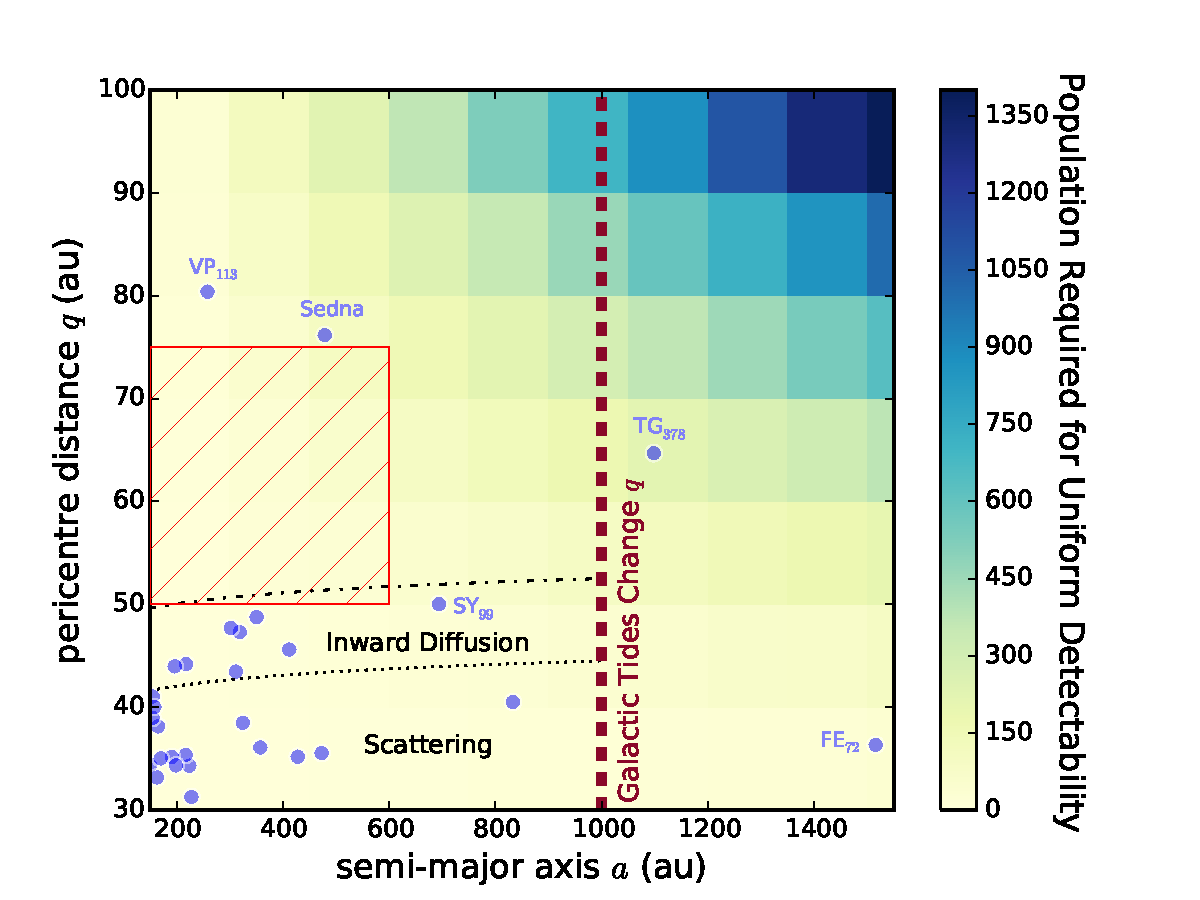
\includegraphics[width=\textwidth]{figure1.pdf}
\caption{Distribution of known TNOs (observed arcs longer than 10 months) with $a > 150$~au and $q > 30$~au in $a$-$q$ (blue dots).  Also shown are the approximate $q$ boundary below which inward diffusion from the $a > 1000$-au (solid vertical line)  is significant and the $q$ boundary below which outward diffusion in $a$ is significant. The grid of numbers indicates the number of objects needed in each orbit group for detection of that orbit to have similar probability to an orbit with $a = 150$, $q = 30$, see text for details.}
\label{fig:bias}
\end{figure}

An important consideration here is that to use the biases in Figure~1 to aid in understanding the structure of the trans-Neptunian region we need to know the full range of orbits, including those with $a< 200$ and $q<40$, detected in a survey as we can then use the relative sensitivity to scale between the regions. 

One point that is worth noting here is the lack of detections in the region showing by the hashed box in Figure~1.  The hashed box region is devoid of known objects but, generally, our sensitivity to orbits in this zone is not lower than that of other zones where a number of detections are available.  This likely indicates that this zone is, indeed, relatively under-populated, an important point in constraining the dynamics of this region of the Solar System.  The apparent paucity of orbits in this zone has been noted previously \citep[e.g.][]{bannister18,sheppard18}, and is discussed further in Section~\ref{sec:diffusion} below.

\section{High-pericentre TNOs} \label{sec:highq}

In recent literature, there has been much discussion of so-called ``extreme TNOs,'' sometimes defined as having $a>250$~au (sometimes $a>150$~au) and $q\gtrsim37$~au \citep{Sheppardetal2016,bannister17}.
This definition is vague and not necessarily dynamically valid; definitions that make use of orbital elements must use the barycentric not the heliocentric orbit (heliocentric orbital elements are what is provided by the Minor Planet Center Database), due to the long-term effect of Jupiter on these distant orbits.
To date, 16  TNOs with $150<a<1000$~au with multi-opposition orbits reported in the Minor Planet Center database have $q>37$~au, mostly with pericentres in the range $37<q<50$~au.
Two of these TNOs have much larger pericentre distances, with $q>75$~au: Sedna ($q=76.19 \pm 0.03$~au, $a=507 \pm 10$~au; \citealt{brownetal04}) and 2012~VP$_{113}$ ($q=80.3^{+1.2}_{-1.6}$~au, $a = 266^{+26}_{-17}$~au; \citealt{trujillosheppard14}). 
These high-pericentre TNOs have recently spawned a flurry of studies on the hypothesis that an undiscovered distant giant planet can be used to explain properties of their orbits. 
In a sign of a vigorously active area of theoretical investigation, a present planet is by no means the only theory to explain these dynamically interesting orbits.

It has been long recognized that the orbital distribution of TNOs can be used to understand the past dynamical history of the Solar System, particularly the outer giant planets \citep{malhotra93,levison08}.
The basic origin story is that TNOs formed in a dynamically cold disk that was disrupted when Neptune migrated, which caused TNOs to be placed into different types of orbits that have since been classified dynamically \citep[see][]{gladman08}.  
Distant, high-$q$ TNOs are difficult to explain in this framework, because they never approach Neptune closely enough to receive dynamical kicks needed to change their orbits, and their large eccentricities preclude formation in-situ.  

A multitude of theories have been proposed to explain the existence of these large-$a$, high-$q$ TNOs.
Simulations that include perturbations by passing stars in the very early Solar System \citep{kenyonbromley04,morbidellilevison04,KaibQuinn2008,Pfalzneretal2018} or within the original Solar birth nebula \citep{brasser12,brasserschwamb15}, or even capture of TNOs from passing star systems \citep{kenyonbromley04,Jilkovaetal2015} are able to produce high-pericentre TNOs on large-$a$ orbits.
Simulations that take into account the gravitational influence of small TNOs have shown the ``inclination instability'' within a massive planetesimal disk can produce high-$q$ TNOs \citep{madigan2016}, and may cause the most massive TNOs to move to the hightest pericentres \citep{Fleisigetal2018}.

Two mechanisms can produce high-$q$ TNOs with only the known giant planets.
Simulations by \citet{bannister17} have shown that chaotic diffusion caused by a combination of Galactic tides and weak gravitational kicks from Neptune can cause objects to migrate from the inner Oort cloud to high-$q$ TNO orbits. 
This diffusion mechanism can possibly explain all the known TNOs except for the two largest $q$ TNOs (see Section~\ref{sec:diffusion}).
TNOs that are captured into Neptune's mean-motion resonances (MMR) may experience Kozai oscillations inside the MMR, and as Neptune migrates outwards they may drop out of the resonance at high-$q$ where the resonance is narrower, and the TNO is then ``fossilized'' on a dynamically detached, long-term stable orbit \citep{gomes03}.
Several non-resonant, stable TNOs have been discovered on high-$q$ orbits near strong resonances, lending observational support to this theory \citep{pike15,lawler18res}.
Simulations show that the mode and timescale of Neptune's migration affects the distribution of these high-$q$ resonant dropouts \citep{Nesvornyetal2016,kaib16}.
While simulations of scattering TNO capture into MMRs show that this can be effective for raising pericentres as high as $q\gtrsim70$~au, this can only happen for scattering TNOs that already have large inclinations \citep{gallardo12} prior to resonant capture, so this cannot be the emplacement mechanism for Sedna and VP$_{113}$ at $i<25^{\circ}$, despite their locations near low-order, distant resonances.  These known gravitational effects rely solely on the known planets of the solar system.

A separate class of hypotheses invoke planetary-mass bodies to raise pericentres.
The possible presence of an additional undiscovered massive, distant planet has been discussed extensively in the literature from the early days of Kuiper Belt discoveries to the present \citep{gladman02,brownetal04,LykawkaMukai2008,soaresgomes13,trujillosheppard14}, and many recent simulations have shown that a distant massive planet would be quite effective at raising the pericentres of large-$a$ TNOs \citep{batyginbrown16,shankman17,lawler2017,Lietal2018}, however, other aspects of the observed Kuiper Belt are solidly inconsistent with this particular planetary scenario \citep{lawler2017,shankman17,shankman17bias}.  
Simulations that include one or more ``rogue planets,'' with masses similar to Earth that are ejected after orbiting in the Kuiper Belt region for a few hundred million years, are also very successful at lifting pericentres for large-$a$ TNOs \citep{gladmanchan06,silsbee18}.
All of these hypotheses for lifting pericentres of distant TNOs have associated simulations modelling a small-body population, produced with many degrees of freedom. 
The critical test for each hypothesis is how well it reproduces the observed TNO population. 
Several of these models are currently providing population outcomes at the level of detail necessary for testing against the observed TNO population.

%%%%%%%%%%%%%%%%%%%%%%%%%%%%%%%%%%%%%%%%%%%%%%%%%%%%%%%%%%%%%%%%%%%%%
\section{Diffusion and motion of large semi-major axes orbits} \label{sec:diffusion}

The nuanced effects of gravitational perturbation from the planets extend over remarkably wide spatial scales and timescales for large semi-major axes orbits, in ways not seen in the inner Solar System.
As initially suggested by \citet{Duncan1987}, each distant encounter of Neptune by a TNO on a near-parabolic $a \gtrsim 100$~au orbit with a perihelion exterior to Neptune will produce an energy change in the TNO's orbit, even for high-$q$ orbits. 
The effect of the energy change at each perihelion passage is a change in the size of the orbit's semimajor axis, while the orbit's perihelion stays constant.
The weak kicks by Neptune at the TNO's perihelion change its orbital $a$ on a timescale $\propto a^{-1/2}$.
As the semimajor axis changes can be modelled as a random walk, with the orbit either becoming larger or decreasing in size with each passage, this change in orbital dimensions for large-$a$ detached TNOs is an example of dynamical diffusion.
It is an effect that occurs purely under the gravitational influence of the known planets.

\citet{bannister17} showed that diffusion is a substantive effect over Gyr for the large-$a$ detached (high-$q$) TNO orbits.
This investigation was prompted by the discovery of 2013 SY$_{99}$ in the course of the OSSOS survey, on an orbit with $q = 50.0$~au, $a = 733 \pm 42$~au.
Since perihelia passages for orbits as large and distant as SY$_{99}$'s are only every 20~kyr, the energy walk requires the passage of Gyr to show changes in orbital semimajor axis.
The semimajor axis of SY$_{99}$ can change by a factor of two over the age of the Solar System, due to the semimajor axis diffusion of 100~au or more that it experiences on Gyr timescales --- despite being fully 20~au separate at perihelia passages with Neptune's orbit.
There were hints of the presence of diffusion in earlier studies of large TNO orbits: \citet{sheppardtrujillo16} noted semimajor axis mobility in the orbit of their discovery 2013~FT$_{28}$ ($q = 43.47 \pm 0.08$~au, $a = 295 \pm 7$~au), and \citet{gallardo12,brasserschwamb15} saw diffusion in their modelling of sub-samples of extreme TNO orbital phase space.
Integrations of the then-known $45<q<50$~au TNOs, with $180 < a < 300$~au, in the presence of the giant planets showed that they exhibit diffusive semimajor axis behaviour \citep{bannister17}. 
Like Sedna and 2012 VP$_{113}$, these orbits are within the placid $a \lesssim 2000$~au region where they are isolated from the Gyr-timescale influence of perturbations by the Galactic tide \citep{brasserschwamb15}.

The evolution of the largest minor planet orbits cannot take place in isolation. 
Orbits at several thousand au start to experience the effects of the Galactic tide, in the inner fringe of the Oort cloud \citep{dones04}.
The population density of the $a \sim 2000$~au region is presently largely mysterious. 
Long-period comets are sourced from several tens of thousands of au more distant, where the influence of the Galactic tide is dominant \cite[e.g.][]{dones04}.
However, the scattering disk has orbits that extend into the inner Oort region, such as that of 2014~FE$_{72}$ ($q = 36.3\pm 0.1$~au, $a=1505\pm 540$~au\footnote{heliocentric JPL Horizons elements from a 1511 day arc, computed 2018-Jun-11.}; \citealt{sheppardtrujillo16}).
Such large-$a$ scattering orbits as FE$_{72}$ provide a conceptual link between the scattering disk and the inner Oort cloud, both past and present.
The emplacement of the scattering disk and its subsequent decay under encounters with Neptune require many millions of minor planets to have been placed on exceptionally large-$a$ orbits \citep{gladman05, levison06}.

The combination of the existence of diffusion in so many of the large-$a$, high-$q$ TNOs and the way in which the scattering disk overlaps with the inner Oort cloud led \citet{bannister17} to the proposal of a mechanism for populating this region, which follows entirely from known physics and the existence of the known planets:
\begin{quote}
An object scatters outward in the initial emplacement of the scattering disk, pushing the semimajor axis of its orbit into the inner fringe of the Oort cloud. At a semimajor axis of a thousand or more au, Galactic tides couple and torque out the orbit's perihelion. Once an object is orbiting with $q = 50$~au and $a\sim1000-2000$~au, it diffuses to a lower-$a$ orbit via planetary energy kicks. A reservoir population of objects must then exist that cycles under diffusion with $q = 40-50$au and $a\sim1000-2500$~au.
\end{quote}
The scattering-to-diffusion scenario made a prediction for future large-$a$ discoveries: 
\begin{quote}
    Our scenario for forming 2013 SY99's orbit does show that for an inner Oort cloud object with $q$ lifted to $\gtrsim 55$~au, diffusion will be too weak to retract the semimajor axis. Thus, future discoveries with $q\sim60$~au should have $a \gtrsim 1000$~au.
\end{quote}
The next year, \citet{sheppard18} reported the discovery of the first TNO with perihelion intermediate between SY$_{99}$ and the two very high-$q$ TNOs (Sedna and VP$_{113}$): 2015 TG$_{387}$ has $q=65 \pm 1$~au. 
Remarkably, TG$_{387}$ has $a = 1190 \pm 70$~au \citep{sheppard18}, in line with the scattering-to-diffusion scenario.
Under the scenario outlined above, its orbit is fossilized. \citet{sheppard18} showed that in the knonw configuration of the solar system, TG$_{387}$'s orbit is presently near-stable. 

Potentially, orbits like TG$_{387}$'s could return to the more actively diffusing part of the proposed cycling population.
If stellar flybys are also modelled, TG$_{387}$'s orbit can have its perihelion driven to lower values of $q \sim 50-55$~au by the combination of tidal and stellar perturbations. In this case, TG$_{387}$'s orbit becomes more actively altering, diffusing in $a$ on order of a hundred au or more \citep{sheppard18}. 

The scattering to diffusion scenario has an inherent limit to the most distant perihelion of orbit it can explain: the kicks from Neptune that permit diffusion to a lower semimajor axis will become too weak. 
Thus, diffusion does not explain the $q \sim 80$~au orbits of VP$_{113}$ and Sedna. 
However, it provides an interesting possibility that explains well the orbits of the remainder of the currently known TNOs in the Solar System as we know it.

%%%%%%%%%%%%%%%%%%%%%%%%%%%%%%%%%%%%%%%%%%%%%%%%%%%%%%%%%%%%%%%%%%%%%
\section{Dynamical effects expected to be imprinted on the distant Kuiper belt by the presence of a massive planet}

In this section, we discuss the results of published n-body simulations that take into account the strong pericentre-raising effects of an additional distant planet.
The presence or absence of a massive, distant planet results in very different orbital distributions for large-$a$ TNOs.  
According to \citet{batyginbrown16}, certain orbits for this distant planet will cause large-$a$, high-$q$ TNOs to have their orbits physically aligned, so the longitude of the ascending node $\omega$, the argument of pericentre $\Omega$, and the longitude of pericentre $\varpi$ will remain confined for all time.
Subsequent simulations have highlighted other effects a massive distant planet would have on this detached TNO population.

\citet{lawler2017} used n-body simulations to create a Kuiper belt analogue in the presence of a distant massive planet and the four known giant planets, focusing on realisitically creating the scattering TNOs using the method of \citet{kaib11b}, including Galactic tides and stellar flybys.  
These simulations showed that a distant massive planet will take an initially dynamically cold distribution of TNOs and raise pericentres and inclinations on Gyr timescales, while creating the scattering disk.
The resulting TNO distributions from these 5-planet emplacement simulations were then compared with a control simulation that included just the known planets \citep{kaib11b}, which have been shown to well-reproduce the orbital properties of the scattering TNOs at all $a$ \citep{shankman13,lawler2018scat}. 
The 5-planet simulations easily produce a large population of high-$q$ TNOs, but simultaneously produce a wide distribution of inclinations, including a large fraction of retrograde scattering and detached TNOs.

\citet{shankman17} showed that the same inclination-raising mechanism will cause all (then) known high-$q$ TNOs to flip to retrograde inclinations on Gyr timescales, thus there should be a nearly equal number of retrograde as prograde high-$q$ TNOs.
They also showed that with such a huge inclination distribution, the detection of just one of these objects, Sedna, requires a massive number of TNOs on similar $a$ and $q$ orbits spread over a range of inclination, implying a total mass of order tens of Earth masses on such obits.
Dynamical simulations of the newly discovered high-$q$ TNO described in \citet{sheppard18} (2015~TG$_{387}$) agree with this inclination-flipping mechanism; they find that a large fraction of clones of 2015~TG$_{387}$ in simulations that include a distant giant planet flip to retrograde orbits on Gyr timescales.

While observational constraints on a large retrograde population are currently weak due to their large predicted distances \citep{lawler2017}, these simulations imply that if there is a giant distant planet, the inclination distribution of high-$q$, large-$a$ TNOs should be nearly isotropic.
The highest-$q$ known TNOs both have $i<25^{\circ}$, so there is little evidence of such a dynamically hot inclination distribution.
Additionally, the masses required for detection of even one high-$q$ isotropic TNO are worryingly high. 

An additional giant planet is one possible way to explain the orbits of high-$q$ TNOs, but some of the other effects it would have on the orbits of TNOs do not appear to agree with observations.
The entire reason that an additional giant planet was proposed was to explain the apparent alignment of the orbital angles of these high-$q$ TNOs, and here we must discuss the complicated and unintuitive biases that are introduced by surveys of this observtionally challenging TNO population.

%%%%%%%%%%%%%%%%%%%%%%%%%%%%%%%%%%%%%%%%%%%%%%%%%%%%%%%%%%%%%%%%%%%%%
\section{Detectibility of orbital effects}

%Because TNOs are detected by reflected light, we are extremely biased against detecting high-$q$ TNOs that never come very close to the Sun.  

All observational surveys contain biases.
But by understanding and carefully keeping track of as many biases as possible, you can understand which types of detections (in this case, orbits) were most unlikely in your survey, and thus which classes of objects represent larger populations than the number of detections in your survey naively suggest.
Accounting for the fraction of time that a given TNO is visible on its orbit and the survey's sky coverage are the biggest effects, and attempts have been made to quantify and account for biases in several TNO surveys at this level
\citep[e.g.][]{schwambetal10,adams14}.

The OSSOS Ensemble of surveys \citep{petit11,alexandersen16,petit17,bannister18} was specifically designed with bias characterization as a top priority, resulting in Survey Simulator software that allows TNO orbital distribution models to be forward-biased by all the characteristics of the survey, including on-sky pointings for each survey block, magnitude limits, detection efficiencies and chip gaps.
The survey also took great pains to track every single TNO that was detected, using careful orbital measurements over 5 months in each discovery year and recovery over $>3$ oppositions \citep{bannister18}, so there is no bias in orbit type, unlike other surveys which preferentially do not track low-$q$ TNOs, or have a high rate of lost TNOs.
Because of this, TNOs that were detected as part of the OSSOS Ensemble can be analysed statistically, and a degree of de-biasing can be achieved for each subpopulation, measuring orbital properties and size distributions \citep{lawler2018}.

%Using the OSSOS Survey Simulator \citep{petit2018,lawler2018}, \citet{lawler2017} show that despite the dramatic differences in predicted orbital distributions, current surveys are unable to distinguish between these two scenarios because all of the difference is in the extremely-hard-to-detect high-$q$ TNO population.
%[not sure what else to write here]

%%%%%%%%%%%%%%%%%%%%%%%%%%%%%%%%%%%%%%%%%%%%%%%%%%%%%%%%%%%%%%%%%%%%%
\subsection{Biases in the angle of pericentre detection in the large-q large-a TNO sample}

Much has been made of the alignment of the pericentre angle of TNOs
with $a>150$~au.  
When all of the high-$q$ TNOs detected in the OSSOS Ensemble are analyzed separately from all other known high-$q$ TNOs, the distribution of orbital angles $\omega$, $\Omega$, and $\varpi$ are consistent with a uniform distribution \citep{shankman17bias,bannister18}.
To restate this a different way, when a uniform distribution of high-$q$, large-$a$ orbits is forward-biased by the OSSOS survey pointings and detection efficiencies, it produces sets of high-$q$, large-$a$ simulated detections that are statistically indistinguishable from the real survey detections.
The high-$q$, large-$a$ TNOs detected by the OSSOS ensemble of surveys show no evidence for orbital clustering.

Many of the high-$q$, $a>150$~au TNOs discovered to date are from surveys that do not report their pointings or tracking fractions, so we cannot statistically test the populations in the same way as the OSSOS detections, but we can make some assumptions about telescope pointings in order to test the biases that are likely present in some of these surveys.
In Figure~\ref{fig:bias_jj} we present the current sample of such
orbits (as of 2018-Oct-1) to allow some examination of that sample.
The figure presents the sample of 6 high-$q$ TNO orbits that created the original
speculation (blue points), the next six TNOs detected (orange
points), and the most recently discovered TNOs in green.  The feature
that originally drew the attention of the discovers \citep{trujillosheppard14} was the lack of detection of
objects with $250^{\circ}< \omega < 60^{\circ}$.  Flux bias in the detected sample
causes most detections to be of objects near the pericentres of the
orbits (i.e.\ with mean anomaly $\mathcal{M}$ near $0^{\circ}$ or $360^{\circ}$).  This is coupled with the
habit of conducting TNO searches in fields that are predominantly
straddle the sky location of the heliocentric plane forces most
discovered objects to have values of $\omega$ near $0^{\circ}$ (or $360^{\circ}$) and $180^{\circ}$ (as described in Section~\ref{sec:intro}).
Although the preference for angles near $360^{\circ}$ is clearly present in the
early sample, there were no detections found near $180^{\circ}$, which is a puzzling feature of the sample.

In Figure~\ref{fig:bias_jj} we also give, on a grid of ($\omega$,$\Omega$) values, the relative
number of detections one might expect at the given $\Omega$,
$\omega$ values when drawing from a sample that is uniformly
distributed but with $a$, $q$, $i$ sampled from the known TNOs.
For simplicity, we assume a flux-limited survey focusing on fields south of the
ecliptic and observing in September, October, November and February
and March (when the best weather conditions occur in the mountains of Chile).  
From the grid of numbers we can see that there are parts
of the ($\Omega$, $\omega$) space that are much more strongly detected than others.  Our
example survey is just provided as thought experiment to alert the
reader to the complexity of the bias interactions. The alignment first
reported is now, largely, washed out by the increased sample size but
there continues to be a paucity of detections near $\omega = 180^{\circ}$.
Without detailed knowledge of the pointing history and careful
measuring of a survey's detection and tracking efficiency through the various seasons of observations,
interpretation of Figure~\ref{fig:bias_jj} is problematic at best.  Regardless of the
distributions physical reality, there are no described gravitational
processes that keep $\omega$ values away from $180^{\circ}$, and
accepting that the distribution is most likely observational biases is
the only supportable explanation.

Subsequent to the claim of an alignment of $\omega$ values, possible
alignment in the longitude of pericentre ($\varpi=\Omega+\omega$) has become
a popular point of discourse,  The appeal being that one can conceive
of physical processes that might align the values of $\varpi$ \citep[e.g.][]{batyginbrown16},
making this a plausibly physical structure.  However, one must
consider that the false (observationally biased) alignment that exists within detected distribution of $\omega$ values
propagates forward into a clustering $\varpi$ as the values of
$\Omega$ are not uncorrelated (see Figure~\ref{fig:bias_jj}).  Thus, although there
are proposed good physical mechanism to cause a clustering or alignment of
$\varpi$ the clustering of the observed values of
$\varpi$ is driven by the same observational biases reported
in the previous paragraph.

\begin{figure}
\centering
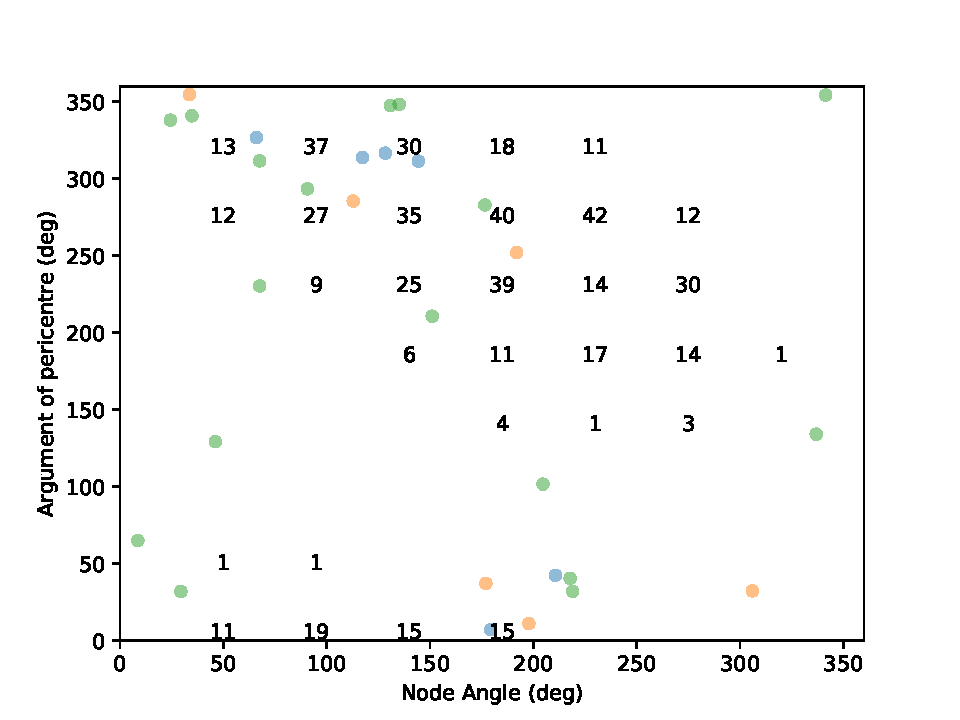
\includegraphics[width=\textwidth]{figure2.pdf}
\caption{Dots show distribution of known TNOs (observed arcs longer than 10 months) with $a > 150$~au and $q > 30$~au in ($\Omega$, $\omega$).  Blue dots indicate the first six such known TNOs, orange dots the next six and the green dots the most recently discovered TNOs.  The lack of objects with values of $\omega$ near $180^{\circ}$ is not an easy bias to disentangle.  The grid of numbers indicate the number of objects a mock survey would have detected on a gird of $\Omega$, $\omega$ values (grid locations without a number had zero (0) detections.  
The shaded boxes show the relative number of detections (linear scale) in the survey described in the text, simulating a southern hemisphere survey, starting from a uniform distribution of ($\Omega$,$\omega$).
The most detectable area of ($\Omega$, $\omega$)-space (darkest purple squares) occurs where most of the first known high-$q$ TNOs are. }
\label{fig:bias_jj}
\end{figure}

%%%%%%%%%%%%%%%%%%%%%%
\section{Summary and Conclusion} 

\subsection{Lack of $50<q<70$~au TNOs is evidence against an additional planet}

The authors of this chapter have already reported some of the problematic orbital evolution effects that a additional massive planet in the outer solar system would create.  In  those works we find that the alignment of orbits is caused by a massive external planet are particularly strong \citep{shankman17}  and the signature of such an alignment would be difficult to detect in the current sample \citep{lawler2017}.  Thus, our expectation is that this process is not at work and there is {\em not} strong evidence of a massive external perturber.

Figure~1, however, provides an intriguing possibility.  We may, in fact, be able to exclude the existence of such a planet with present datasets. From the figure one can see that there are no objects with pericentres between 50 and 80 au and semi-major axis inerior to 1000~au.  Indeed, other authors have already remarked on the absence of such orbits \citep[e.g.][]{sheppard18,bannister17}.  Recall that in Figure~1 the grid of numbers provides some measure of the inverse probability of detection of particular obits, given a survey.  A survey that might have detected an object at $a \sim 500$ and $q \sim75$ is actually more likely to have detected objects with similar $a$ but smaller values of $q$, the same is true of the other $q>70$ detections, the lower-$q$ but similar $a$ detections are always more likely.  Thus, the lack of detections in the $50 < q < 70$~au range may be indicating that there really are not objects on orbits in this range.  This strongly contradicts models of orbital evolution that include a massive external planet as the gravitational action of such an object invariably drags many objects from below and above this zone into it.  Thus, if the lack of objects in $50 < q < 70$~au range is real, and currently the evidence suggests that it is, the hypothesized external planet can be excluded\footnote{there may be some very specialized orbital configuration that preserves the emptiness of this  $q$ zone but, as of this writing, none have been proposed}.

\subsection{The orbits of Sedna and 2012 VP$_{113}$ are weird}

There are several effects that can raise pericentres, but raising them
to such large values is {\em hard}.  
A distant massive planet doesn't actually help this; sure it's great
at raising pericentres, but it also causes inclinations to become huge
and we see no evidence for that.  The notable lack of TNOs with pericentres in the range $50<q<70$~au while there are two known TNOs with $q>70$~au also does not fit with 
the dynamical influence wielded by a distant planet, which would cause TNOs to be distributed across a range of $q$ values at any given moment.
Except for Sedna and VP$_{113}$, all
of the existing high-$q$ TNOs can be explained by other dynamical
mechanisms that do not require an additional giant planet.  Even the
newest announced high-$q$ TNO, 2015~TG$_{387}$, perfectly falls into
the $a$, $q$ range predicted to be affected by chaotic diffusion as
described in \citet{bannister17}.

Rogue planets are an intriguing possibility that appear to create distributions of high-$q$ TNOs that match observations reasonably well \citep{lawler2018,silsbee18}, and precursor simulations like \citet{gladmanchan06} should be revisited in light of
the new high-$q$ TNO discoveries to date.  These types of simulations
produce Sedna-like TNOs without a worryingly large retrograde TNO population at large-$a$, as is produced by a massive distant planet remaining in orbit to this day.

% \bibliographystyle{apj}
\bibliography{citations}

%% This command is needed to show the entire author+affilation list when
%% the collaboration and author truncation commands are used.  It has to
%% go at the end of the manuscript.
%\allauthors

%% Include this line if you are using the \added, \replaced, \deleted
%% commands to see a summary list of all changes at the end of the article.
%\listofchanges

\end{document}

% End of file `sample62.tex'.
